\documentclass[11pt,a4paper,fontset=fandol]{ctexart}

\usepackage[a4paper,margin=1in]{geometry}
\usepackage{graphicx}
\usepackage{booktabs}
\usepackage{array}
\usepackage{float}
\usepackage{hyperref}

\hypersetup{hidelinks}
\renewcommand{\arraystretch}{1.15}
\setlength{\parindent}{2em}
\setlength{\parskip}{0.35em}
\setlength{\emergencystretch}{3em}

\title{\textbf{SimCLR 数据增强消融实验简报}\\
\large 基于 CIFAR-10 子集的 100 Epoch 对比分析}
\author{}
\date{}

\begin{document}

\maketitle
\thispagestyle{empty}

\begin{abstract}
本文将仓库中的 README 与实验结果文件压缩整理为一份短论文式报告，讨论在 CIFAR-10 的 5000 张训练样本子集上，不同数据增强组件对 SimCLR 表示学习效果的影响。实验比较了四种增强方案：完整增强流水线（\texttt{baseline}）、去掉高斯模糊（\texttt{no\_blur}）、去掉颜色扰动（\texttt{no\_color\_jitter}）和去掉随机灰度化（\texttt{no\_grayscale}）。所有实验均在相同设置下使用 ResNet-18 训练 100 个 epoch，并通过冻结编码器的线性评估检验下游分类表现。结果显示，\texttt{no\_color\_jitter} 在对比学习训练指标上显著领先，但在线性评估中反而最差；相反，\texttt{no\_grayscale} 和 \texttt{no\_blur} 的下游精度都优于 \texttt{baseline}。这一结果说明，SimCLR 预训练阶段的优化指标并不能直接作为表示质量的可靠代理。
\end{abstract}

\section{引言}
本次实验关注一个非常具体的问题：在其他训练条件保持不变的前提下，\texttt{ColorJitter}、\texttt{GaussianBlur} 和 \texttt{RandomGrayscale} 这三个常见增强组件，究竟如何影响 SimCLR 的预训练表现，以及更重要的下游分类效果。这个问题看似简单，但它直接关系到我们应当如何理解对比学习中的“训练得更好”。

仓库中的原始 README 已经给出了完整实验记录，但其中既包含报告性内容，也包含交接与复现信息。为了让结论更适合展示，这里将信息重新组织为论文式结构，突出研究问题、实验设置、结果比较和方法论结论。

\section{实验设置}
实验数据集为 CIFAR-10，主干网络为 ResNet-18，projection head 维度为 128。所有实验统一使用 batch size 256、temperature 0.07、learning rate 0.0003、weight decay $1\times10^{-4}$、每张图像 2 个 views、随机种子 0，并训练 100 个 epoch。为了控制成本，本次预训练只使用 5000 张训练图像，运行设备为 CPU，data loader workers 设为 0。

下游评估采用冻结编码器加线性分类器的方式，在 5000 张 CIFAR-10 训练图像上训练线性层，并在 10000 张测试图像上报告测试精度。这样的设置可以较直接地反映预训练表示是否真正有利于分类任务。

基线增强流水线为：
\begin{quote}
\small\ttfamily
RandomResizedCrop + RandomHorizontalFlip +\\
RandomApply(ColorJitter, p=0.8) + RandomGrayscale(p=0.2) +\\
GaussianBlur + ToTensor
\end{quote}

本次消融每次只改动其中一个组件，因此四组实验之间的主要差异只来自增强策略本身。

\section{结果}

\subsection{预训练阶段结果}
表~\ref{tab:pretrain} 汇总了四组实验在 SimCLR 训练结束时的核心指标。若只看对比学习任务自身，\texttt{no\_color\_jitter} 的表现几乎是压倒性的：它的最终 loss 最低，contrastive top-1 和 top-5 也显著高于其他方案。

\begin{table}[H]
\centering
\small
\caption{SimCLR 预训练阶段最终指标}
\label{tab:pretrain}
\begin{tabular}{lccc}
\toprule
增强方案 & Final loss & Contrastive top-1 & Contrastive top-5 \\
\midrule
\texttt{baseline} & 3.892488 & 28.4951 & 46.2685 \\
\texttt{no\_blur} & 3.783522 & 30.0884 & 47.9235 \\
\texttt{no\_color\_jitter} & 1.784125 & 63.2299 & 80.0781 \\
\texttt{no\_grayscale} & 3.476313 & 30.7771 & 51.7167 \\
\bottomrule
\end{tabular}
\end{table}

\noindent\small 注：这里的 contrastive top-1 / top-5 反映的是对比学习任务内部把正样本排到前列的能力，并不是 CIFAR-10 分类准确率。\normalsize

\begin{figure}[H]
\centering
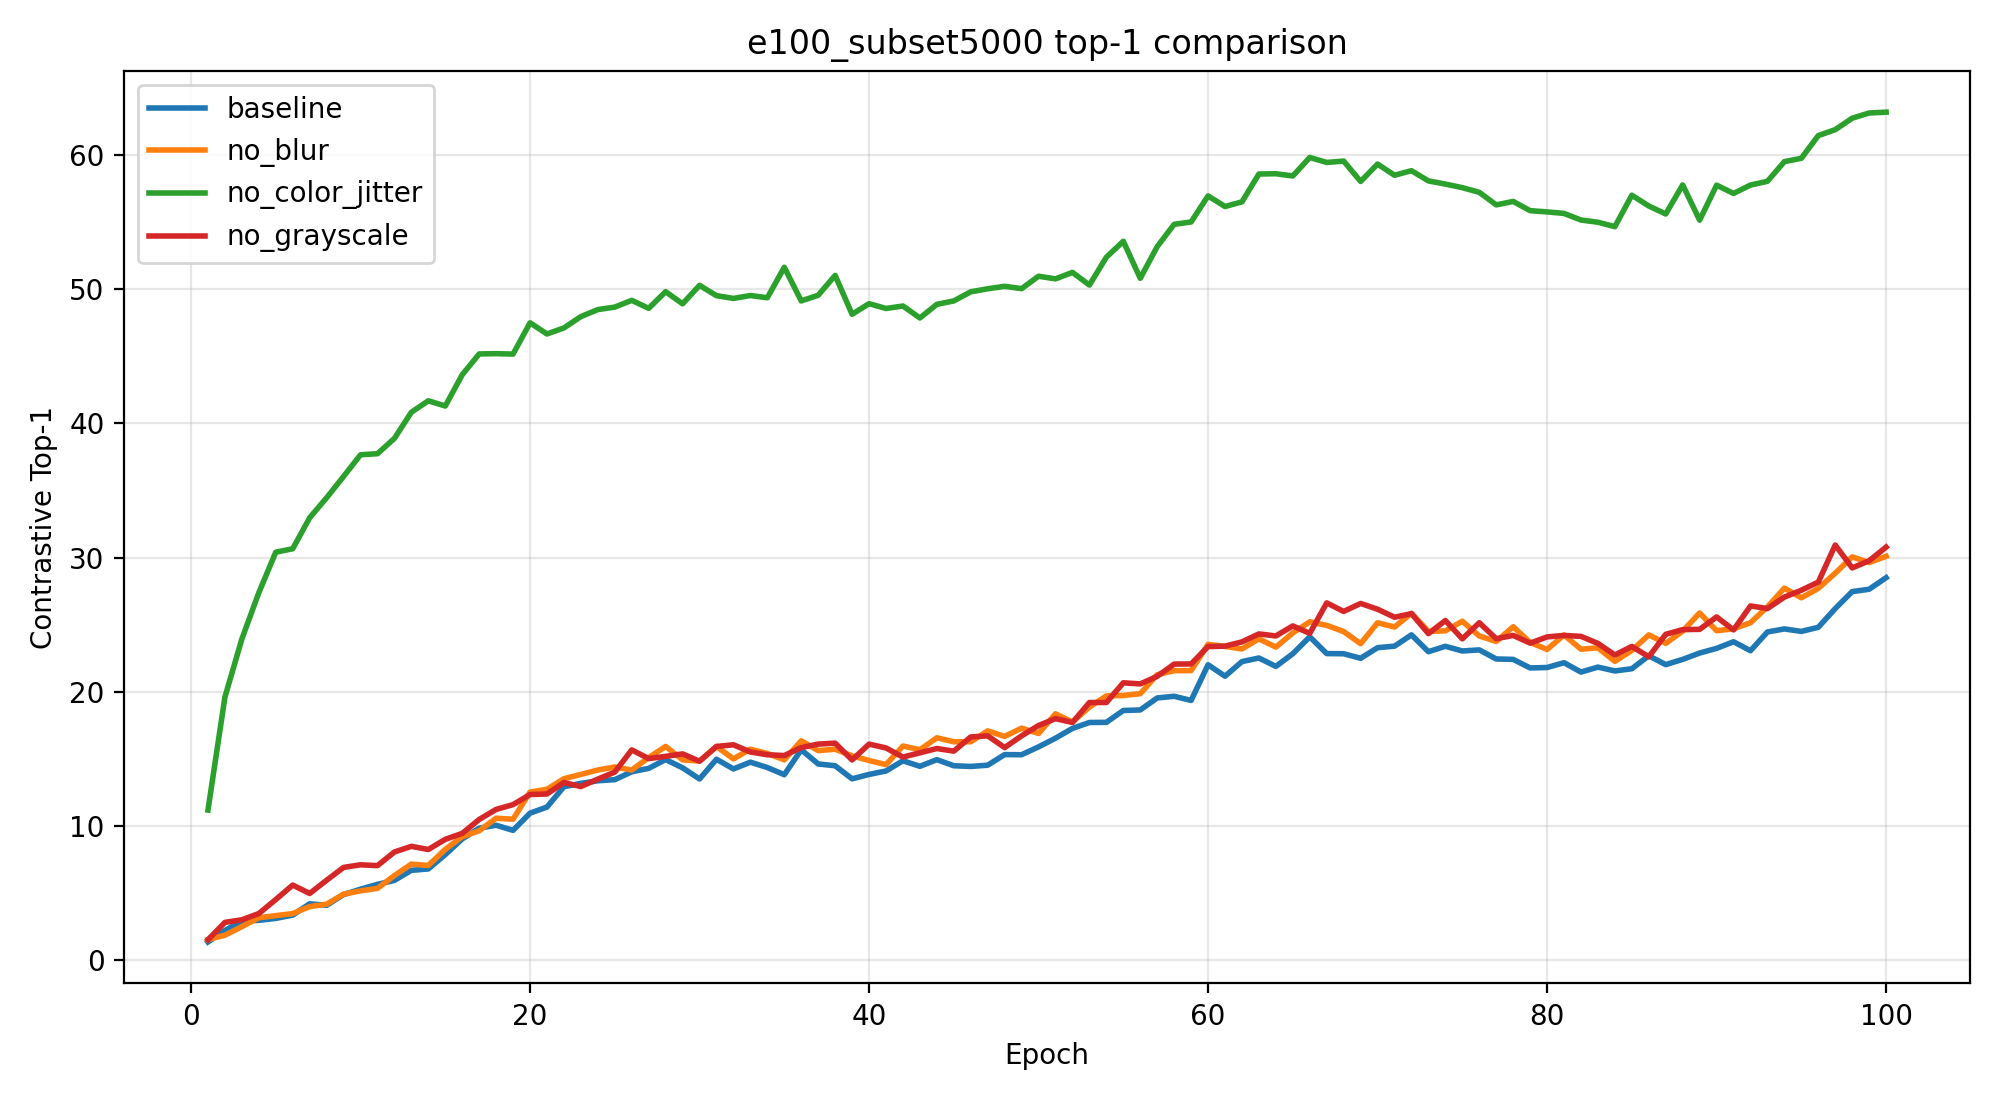
\includegraphics[width=0.48\linewidth]{../outputs/augmentation_suite/e100_subset5000_accuracy_vs_epoch_comparison.png}
\hfill
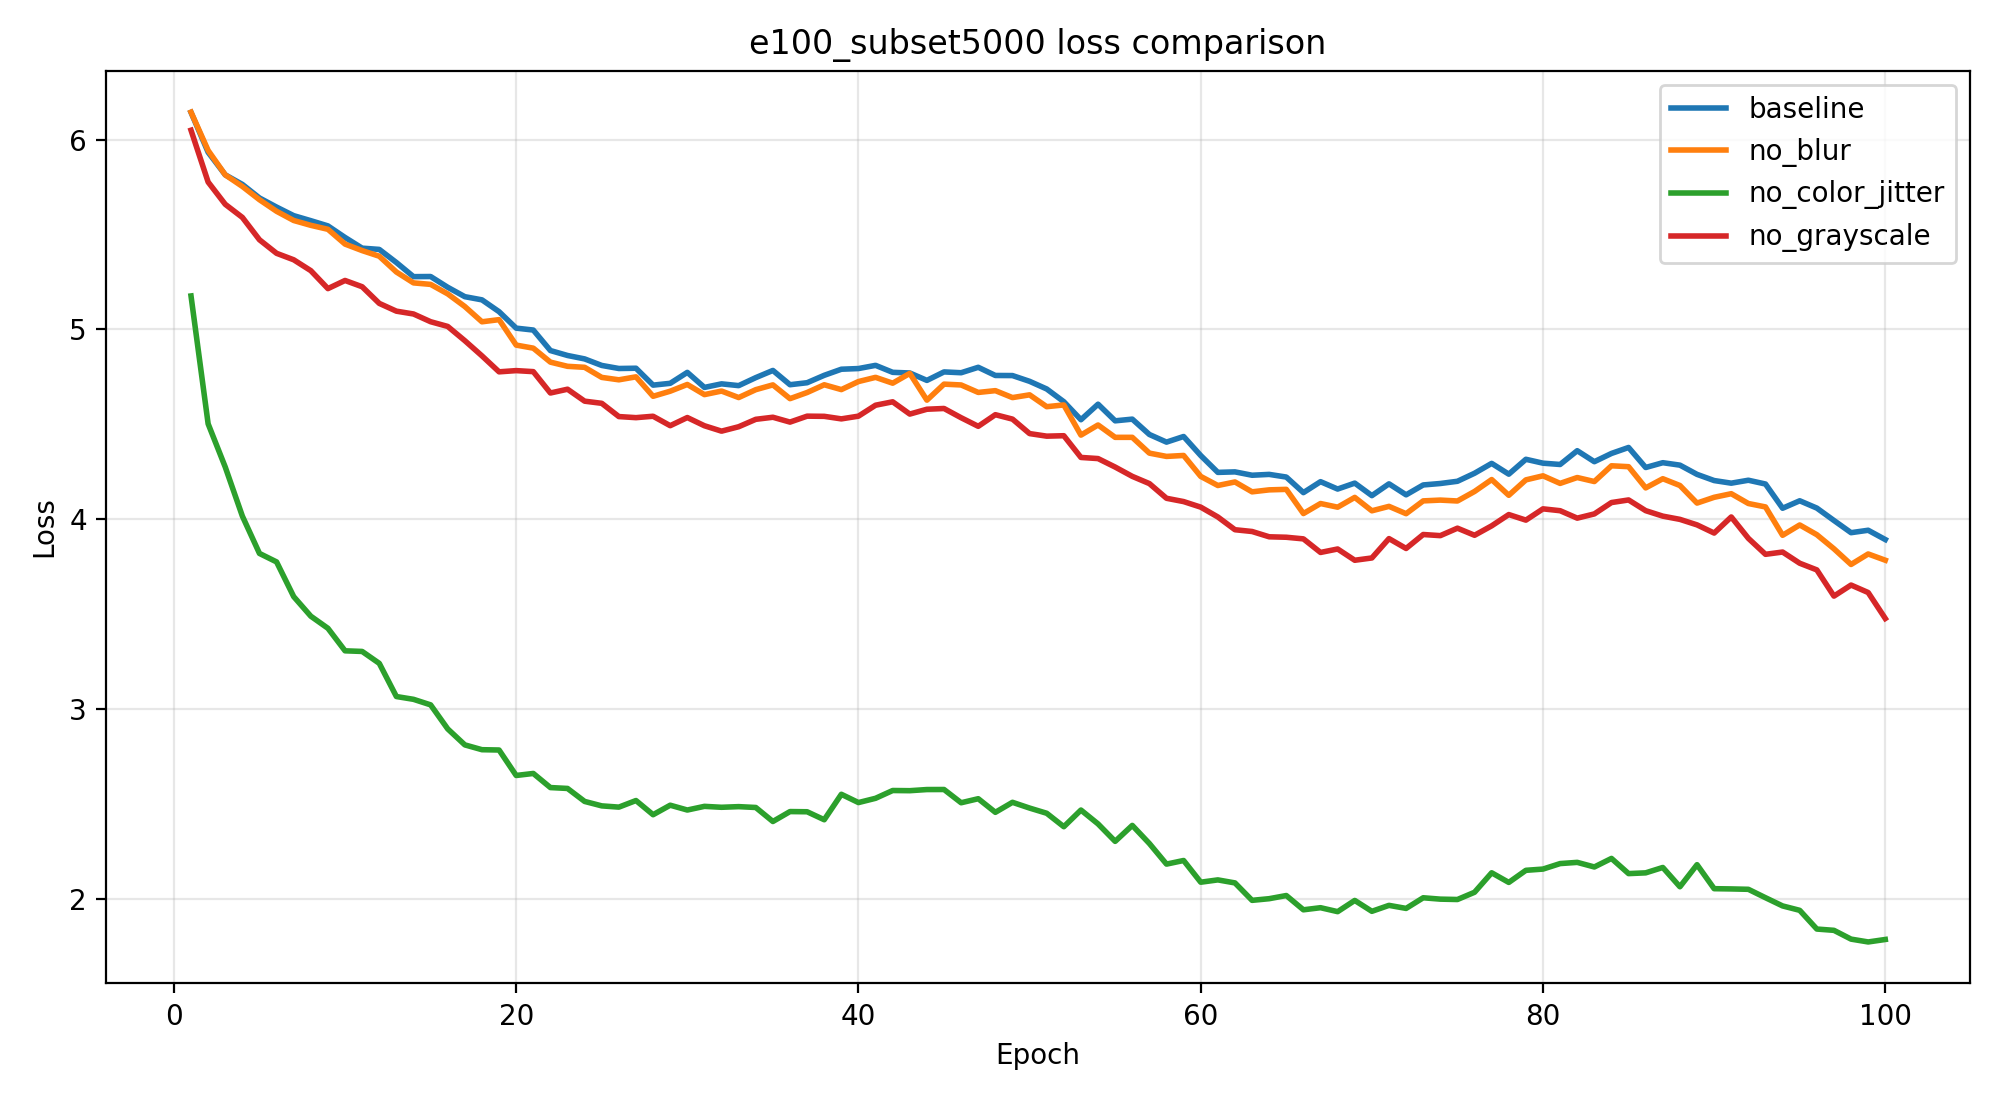
\includegraphics[width=0.48\linewidth]{../outputs/augmentation_suite/e100_subset5000_loss_vs_epoch_comparison.png}
\caption{四组增强方案在预训练阶段的 contrastive top-1 与 loss 变化曲线}
\label{fig:pretrain_curves}
\end{figure}

从图~\ref{fig:pretrain_curves} 可以进一步看到，\texttt{no\_color\_jitter} 在整个训练过程中都拥有更快的收敛速度和更高的对比学习指标。如果只停留在预训练阶段，我们很容易得出“去掉颜色扰动更好”的结论。

\subsection{线性评估结果}
真正关键的结果出现在下游线性评估中，如表~\ref{tab:linear_eval} 所示。最佳 test accuracy 来自 \texttt{no\_grayscale}，达到 44.92\%，比 \texttt{baseline} 的 43.57\% 提高了 1.35 个百分点；\texttt{no\_blur} 也达到 44.56\%，比基线高 0.99 个百分点。相反，训练指标最亮眼的 \texttt{no\_color\_jitter} 测试精度只有 42.07\%，反而比基线低了 1.50 个百分点。

\begin{table}[H]
\centering
\small
\caption{冻结编码器线性评估结果}
\label{tab:linear_eval}
\begin{tabular}{lccc}
\toprule
增强方案 & Train accuracy & Test accuracy & Test top-5 \\
\midrule
\texttt{baseline} & 71.50 & 43.57 & 89.63 \\
\texttt{no\_blur} & 71.90 & 44.56 & 89.78 \\
\texttt{no\_color\_jitter} & 71.48 & 42.07 & 88.47 \\
\texttt{no\_grayscale} & 72.94 & 44.92 & 89.62 \\
\bottomrule
\end{tabular}
\end{table}

\begin{figure}[H]
\centering
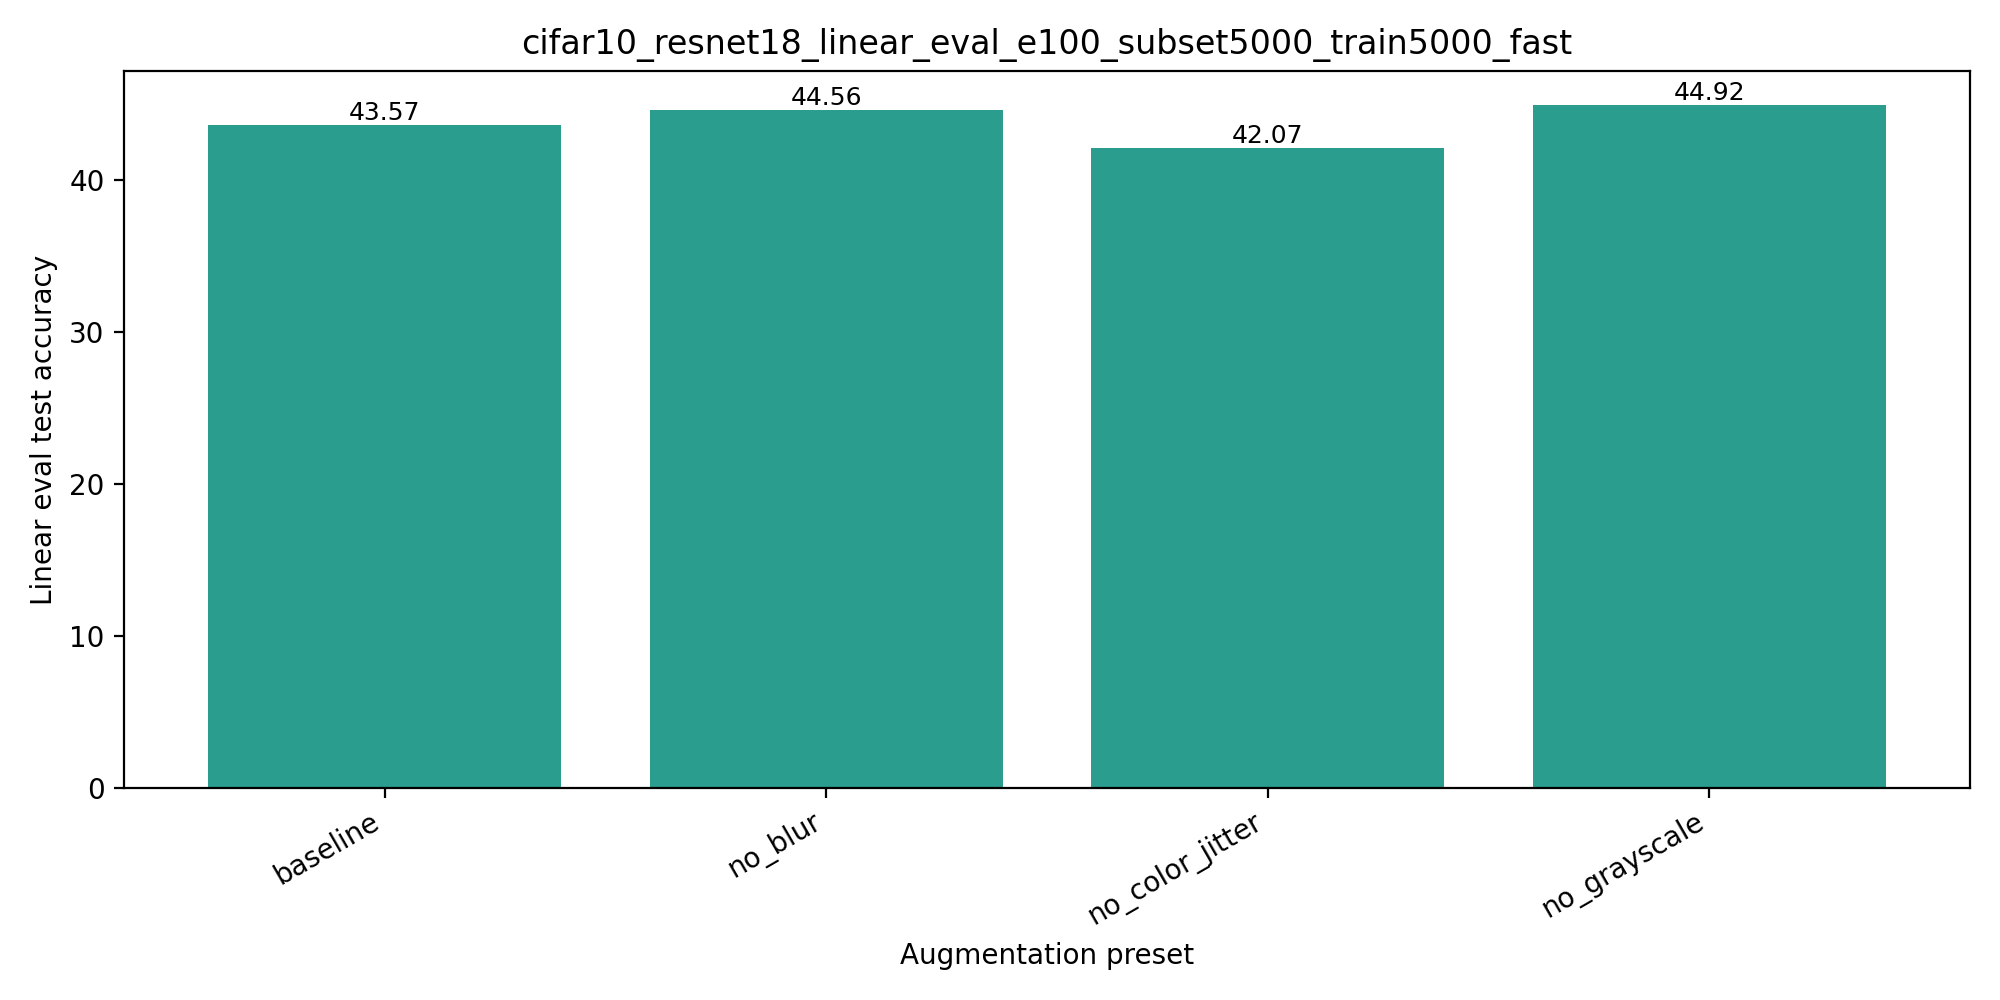
\includegraphics[width=0.78\linewidth]{../outputs/linear_eval/cifar10_resnet18_linear_eval_e100_subset5000_train5000_fast_test_accuracy.png}
\caption{冻结编码器线性评估的测试精度对比}
\label{fig:linear_eval}
\end{figure}

图~\ref{fig:linear_eval} 将这种反差展示得更加直接：\texttt{no\_color\_jitter} 虽然“更会做预训练任务”，但并没有学到更适合分类的表示；\texttt{no\_grayscale} 和 \texttt{no\_blur} 的对比学习指标并不夸张，却在下游任务中更可靠。

\section{讨论}
这组实验最有价值的地方，不是简单地告诉我们“哪一种增强组合赢了”，而是揭示了预训练目标与下游目标之间可能存在明显错位。\texttt{no\_color\_jitter} 是最典型的反例：当颜色扰动被移除之后，对比学习任务本身可能变得更容易，模型也因此更容易把正样本配对成功，于是 loss 更低、top-1 和 top-5 更高；但与此同时，模型学到的表示可能更依赖颜色线索，缺少了对颜色变化的鲁棒性，最终不利于分类泛化。

相比之下，\texttt{RandomGrayscale} 和 \texttt{GaussianBlur} 在这组设置里并没有体现出必要性，甚至略微拖累了最终测试精度。至少在 CIFAR-10、ResNet-18、100 epoch、5000 样本子集这一条件下，去掉灰度增强和去掉模糊增强都比保留完整基线更稳妥。

当然，这些结论也有边界：本次实验只使用单一随机种子，只覆盖 CIFAR-10 的 5000 样本子集，并且在 CPU 环境下完成训练。因此，这里的结果更适合作为当前设置下的经验结论，而不是对所有 SimCLR 场景的一般定律。

\section{结论}
在本次实验设置下，若需要从四个编码器中优先选择后续下游任务的候选，推荐顺序为 \texttt{no\_grayscale}、\texttt{no\_blur}、\texttt{baseline}、\texttt{no\_color\_jitter}。更重要的是，这份实验给出的核心方法论结论非常明确：\textbf{SimCLR 训练阶段的优化指标和下游迁移效果之间，可能出现显著不一致，因此不能只凭预训练 loss 或 contrastive top-k 指标判断表示质量。}

\section{复现实验入口}
如需继续扩展本实验，仓库中的 \path{run_augmentation_suite.py} 用于批量运行增强消融，\path{plot_augmentation_training_comparison.py} 用于生成跨实验训练对比图，\path{run_linear_eval_suite.py} 用于执行冻结编码器线性评估并汇总结果。本文中的所有数值均来自仓库现有的 \path{summary.json}、\path{metrics.csv} 和线性评估汇总文件。

\end{document}
